\documentclass[aspectratio=169]{beamer}
%
% Choose how your presentation looks.
%
% For more themes, color themes and font themes, see:
% http://deic.uab.es/~iblanes/beamer_gallery/index_by_theme.html
%
\mode<presentation>
{
  \usetheme{metropolis}      % or try Darmstadt, Madrid, Warsaw, ...
  \usecolortheme{default} % or try albatross, beaver, crane, ...
  \usefonttheme{structurebold}  % or try serif, structurebold, ...
  \setbeamercolor{background canvas}{bg=white}
  \setbeamertemplate{navigation symbols}{}
  \setbeamertemplate{bibliography item}{\insertbiblabel}
  %\setbeamertemplate{caption}[numbered]
} 
\usepackage[english]{babel}
\usepackage[utf8x]{inputenc}
\usepackage{listings}             % Include the listings-package
\usepackage{bm}	% math package

\hypersetup{
    colorlinks = true,
    linkcolor = {black},
    urlcolor = {blue}
}

\DeclareMathOperator*{\argmin}{arg\,min}

\title[Deep Learning and Temporal Data Processing]{Deep Learning and Temporal Data Processing}
\subtitle{3 - Recurrent Neural Networks}
\institute{University of Modena and Reggio Emilia}
\author{Andrea Palazzi}
%\date{June 21th, 2017}

\def\thisframelogos{}

\newcommand{\framelogo}[1]{\def\thisframelogos{#1}}

\addtobeamertemplate{frametitle}{}{%
\begin{tikzpicture}[remember picture,overlay]
\node[anchor=north east] at (current page.north east) {%
    \foreach \img in \thisframelogos {%
        %\hspace{.5ex}%
        \includegraphics[height=3.5ex]{\img}%
    }%
};
\end{tikzpicture}}

\begin{document}

\framelogo{img/template/logo_unimore_white.png}

\bgroup
\renewcommand{\insertframenumber}{}
\begin{frame}[noframenumbering]
  \titlepage
\end{frame}
\egroup
\begin{frame}{Agenda}
  \tableofcontents
\end{frame}


%%%%%%%%%%%%%%%%%%%%%%%%%%%%%%%%%%%%%%%%%%%%%%%%%%%%%%%%%%%%%%%%%%
%%%%%%%%%%%%%%%%%%%%%%%%%%%%%%%%%%%%%%%%%%%%%%%%%%%%%%%%%%%%%%%%%%
%%%%%%%%%%%%%%%%%%%%%%%%%%%%%%%%%%%%%%%%%%%%%%%%%%%%%%%%%%%%%%%%%%

\section{Introduction}

%%%%%%%%%%%%%%%%%%%%%%%%%%%%%%%%%%%%%%%%%%%%%%%%%%%%%%%%%%%%%%%%%%

\begin{frame}{Recurrent Neural Networks}
In \textbf{feedforward neural network} computation flows directly from input $\bm{x}$ through intermediate layers $\bm{h}$ to output $\bm{y}$.\\
\vspace{0.5cm}
Conversely, some networks topology feature feedback connections, in other words model outputs are fed back into the model itself.\\
\vspace{0.5cm}
The term \textbf{recurrent neural networks} defines this family of models.

\end{frame}

%%%%%%%%%%%%%%%%%%%%%%%%%%%%%%%%%%%%%%%%%%%%%%%%%%%%%%%%%%%%%%%%%%

\begin{frame}{Recurrent Neural Networks}
Recurrent neural networks (RNN) are \textbf{specialized for processing sequences}. Similarly, we saw that convolutional neural networks feature specialized architecture for processing images.\\
\vspace{0.4cm}
RNNs boast a \textbf{much wider API with respect to feedforward neural networks}. Indeed, these models can deal with \textit{sequences} in the input, in the output or even both.
\begin{figure}
\begin{tabular}{c}
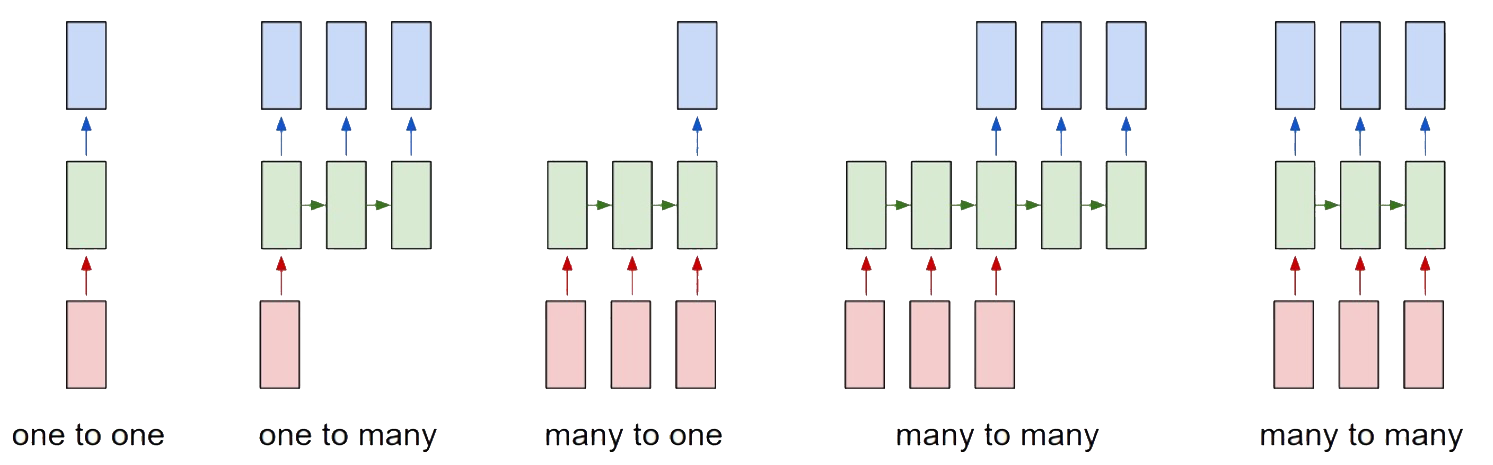
\includegraphics[width=0.8\textwidth]{img/rnn/rnn_api.png}
\end{tabular}
\end{figure}
\end{frame}

%%%%%%%%%%%%%%%%%%%%%%%%%%%%%%%%%%%%%%%%%%%%%%%%%%%%%%%%%%%%%%%%%%
%%%%%%%%%%%%%%%%%%%%%%%%%%%%%%%%%%%%%%%%%%%%%%%%%%%%%%%%%%%%%%%%%%
%%%%%%%%%%%%%%%%%%%%%%%%%%%%%%%%%%%%%%%%%%%%%%%%%%%%%%%%%%%%%%%%%%
\section{Vanilla RNN}

\begin{frame}{Vanilla RNN}
\begin{columns}
\begin{column}{0.3\textwidth}
\begin{tabular}{c}
	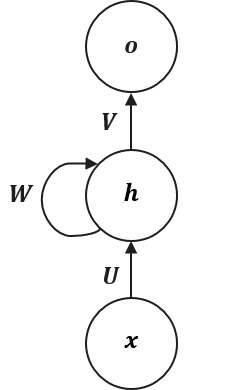
\includegraphics[width=0.7\textwidth]{img/rnn/vanilla_rnn.png}
\end{tabular}
\end{column}
\begin{column}{0.7\textwidth}
The vanilla RNN is provided with three sets of parameters:
\begin{itemize}
	\item $\bm{U}$ maps inputs to the hidden state
	\item $\bm{W}$ parametrizes hidden state transition
	\item $\bm{V}$ maps hidden state to output 
\end{itemize}
\vspace{0.5cm}
System dynamics is as simple as:
\begin{equation}
	\begin{cases}
	\bm{h}^{(t)} = \phi(\bm{W}\,\bm{h}^{(t-1)} + \bm{U}\,\bm{x}^{(t)})\\
	\bm{o}^{(t)} = \bm{V}\,\bm{h}^{(t)}
	\end{cases}
\end{equation}
\end{column}
\end{columns}
\end{frame}

%%%%%%%%%%%%%%%%%%%%%%%%%%%%%%%%%%%%%%%%%%%%%%%%%%%%%%%%%%%%%%%%%%

\begin{frame}{Intuition about Hidden State}
\begin{columns}
\begin{column}{0.3\textwidth}
\begin{tabular}{c}
	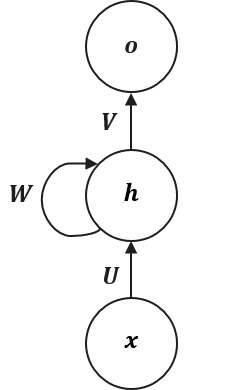
\includegraphics[width=0.7\textwidth]{img/rnn/vanilla_rnn.png}
\end{tabular}
\end{column}
\begin{column}{0.7\textwidth}
The hidden state $\bm{h}^{(t)}$ can be intuitively viewed as a \textit{lossy} summary of the sequence of past inputs fed to the network, in which are stored the main task-relevant aspects of the past sequence of inputs up to time $t$.\\
\vspace{0.5cm}
Since the an input sequence of arbitrary length $(\bm{x}^{(1)}, \bm{x}^{(2)}, ..., \bm{x}^{(t)})$ is mapped into a fixed size vector $\bm{h}^{(t)}$, this summary is necessarily lossy.
\end{column}
\end{columns}
\end{frame}

%%%%%%%%%%%%%%%%%%%%%%%%%%%%%%%%%%%%%%%%%%%%%%%%%%%%%%%%%%%%%%%%%%
%%%%%%%%%%%%%%%%%%%%%%%%%%%%%%%%%%%%%%%%%%%%%%%%%%%%%%%%%%%%%%%%%%
%%%%%%%%%%%%%%%%%%%%%%%%%%%%%%%%%%%%%%%%%%%%%%%%%%%%%%%%%%%%%%%%%%

\section{Training a RNN}

\begin{frame}{Unfolding the Computational Graph}
A recurrent computational graph can be unfolded into a sequential computational graph with a repetitive structure.
\begin{equation*}
\bm{h}^{(t)} = f(\bm{h}^{t-1}, \bm{x}^{(t)}; \bm{\theta})
\end{equation*}
\begin{figure}
\begin{tabular}{c}
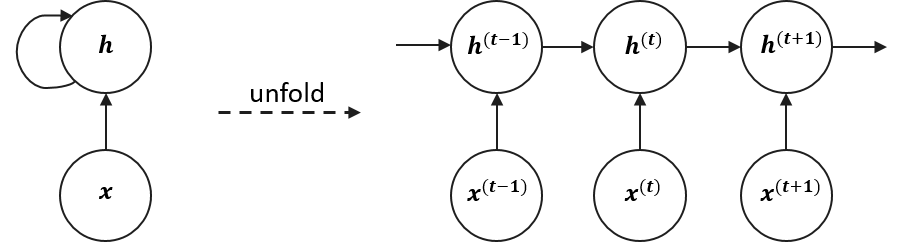
\includegraphics[width=0.8\textwidth]{img/rnn/rnn_unfold.png}
\end{tabular}
\end{figure}
\begin{columns}
\end{columns}
\end{frame}

%%%%%%%%%%%%%%%%%%%%%%%%%%%%%%%%%%%%%%%%%%%%%%%%%%%%%%%%%%%%%%%%%%

\begin{frame}{Backpropagation Through Time}
The capacity to \textbf{unfold a recurrent graph into a DAG} (Directed Acyclic Graph) allows to train recurrent neural network by means of standard backpropagation.\\
\vspace{0.5cm}
Because the gradient conceptually flows backward though time instead of though layers, this algorithm is usually referred to as \textbf{backpropagation through time (BPTT)}.
\end{frame}

%%%%%%%%%%%%%%%%%%%%%%%%%%%%%%%%%%%%%%%%%%%%%%%%%%%%%%%%%%%%%%%%%%

\begin{frame}{Backpropagation Through Time}
Let's make an example for an simple architecture which processes sequences of length $\tau=3$ and produces an output at the end of the sequence.
\begin{figure}
\begin{tabular}{c}
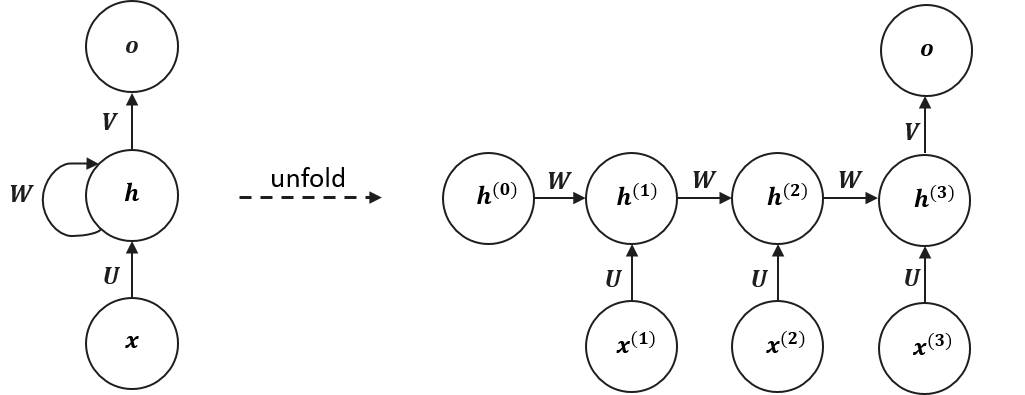
\includegraphics[width=0.8\textwidth]{img/rnn/bptt.png}
\end{tabular}
\end{figure}
\end{frame}

%%%%%%%%%%%%%%%%%%%%%%%%%%%%%%%%%%%%%%%%%%%%%%%%%%%%%%%%%%%%%%%%%%

\begin{frame}{Backpropagation Through Time}
Now, given a differentiable loss on final output $L(\bm{y}, \bm{o})$ let's compute the derivative of the objective $L$ with respect to the weights $\bm{V}$, $\bm{W}$ and $\bm{U}$ and see what happens.
\vspace{0.5cm}
\begin{columns}
\begin{column}{0.5\textwidth}
\begin{figure}
	\begin{tabular}{c}
		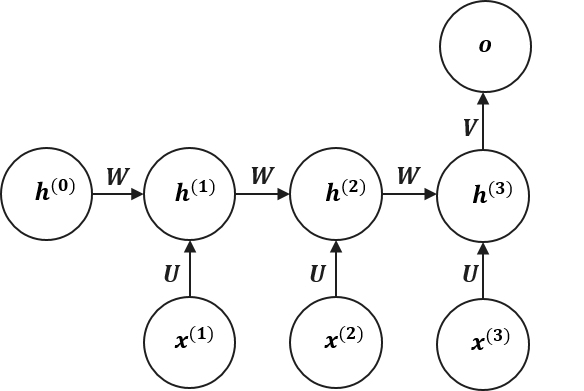
\includegraphics[width=0.8\textwidth]{img/rnn/bptt_unroll.png}
	\end{tabular}
\end{figure}
\end{column}
\begin{column}{0.5\textwidth}
\begin{itemize}
\item $\frac{\partial L}{\partial \bm{V}} = \frac{\partial L}{\partial \bm{o}} \frac{\partial \bm{o}}{\partial \bm{V}}$
\item $\frac{\partial L}{\partial \bm{W}} = \frac{\partial L}{\partial \bm{o}} \frac{\partial \bm{o}}{\partial \bm{h}^{(3)}} \sum_{k=0}^{3}\left(\frac{\partial \bm{h^{(3)}}}{\partial \bm{h}^{(k)}}\frac{\partial \bm{h}^{(k)}}{{\partial \bm{W}}}\right)$
\item $\frac{\partial L}{\partial \bm{U}} = \frac{\partial L}{\partial \bm{o}} \frac{\partial \bm{o}}{\partial \bm{h}^{(3)}} \sum_{k=0}^{3}\left(\frac{\partial \bm{h^{(3)}}}{\partial \bm{h}^{(k)}}\frac{\partial \bm{h}^{(k)}}{{\partial \bm{U}}}\right)$
\end{itemize}
\vspace{0.5cm}
\textbf{Consideration}: while $\frac{\partial L}{\partial \bm{V}}$ depends only on current state, $\frac{\partial L}{\partial \bm{W}}$ and $\frac{\partial L}{\partial \bm{U}}$ depend on all previous sequence states.
\end{column}
\end{columns}
\end{frame}

%%%%%%%%%%%%%%%%%%%%%%%%%%%%%%%%%%%%%%%%%%%%%%%%%%%%%%%%%%%%%%%%%%

\begin{frame}{The Challenge of Long-Term Dependencies}
Looking closer, we see that terms $\frac{\partial \bm{h^{(t)}}}{\partial \bm{h}^{(k)}}$ must be themselves computed through the chain rule. For example, we can obtain $\frac{\partial \bm{h^{(3)}}}{\partial \bm{h}^{(1)}} = \frac{\partial \bm{h^{(3)}}}{\partial \bm{h}^{(2)}} \frac{\partial \bm{h^{(2)}}}{\partial \bm{h}^{(1)}}$.\\
\vspace{0.5cm}
Turns out \cite{pascanu2013difficulty} that when using \textit{tanh} and \textit{sigmoid} activations, the 2-norm of these Jacobian matrices is upper bounded by $1$ and $1/4$ respectively. Thus, we can easily end up multiplying smaller and smaller numbers until the gradients become zero.\\
\vspace{0.5cm}
This problem is known as \textbf{vanishing gradient problem}, and causes serious trouble when trying to learn long-term dependencies in the input sequences, because contributions of "far-away" steps become zero.
\end{frame}

%%%%%%%%%%%%%%%%%%%%%%%%%%%%%%%%%%%%%%%%%%%%%%%%%%%%%%%%%%%%%%%%%%

\begin{frame}{The Challenge of Long-Term Dependencies}
Depending on the network parameters and choice of activation functions, the opposite problem can arise. This is called \textbf{exploding gradient problem} and happens when gradients become bigger and bigger until numerical problems destroy the optimization process.\\
\vspace{0.5cm}
Both issues can be mitigated through proper weight initialization, accurate choice of activation functions and gradient clipping.\\
\vspace{0.5cm}
\textbf{Note}: these problems can also happen in deep feedforward networks: however, they are more common in recurrent architectures because these models are usually very deep (actually as deep as the length of the input sequence).
\end{frame}

%%%%%%%%%%%%%%%%%%%%%%%%%%%%%%%%%%%%%%%%%%%%%%%%%%%%%%%%%%%%%%%%%%
%%%%%%%%%%%%%%%%%%%%%%%%%%%%%%%%%%%%%%%%%%%%%%%%%%%%%%%%%%%%%%%%%%
%%%%%%%%%%%%%%%%%%%%%%%%%%%%%%%%%%%%%%%%%%%%%%%%%%%%%%%%%%%%%%%%%%
\section{Advanced RNN Architectures}

\begin{frame}{Advanced Recurrent Architectures}
\textbf{Long Short-Term Memory (LSTM)} and \textbf{Gated Recurrent Unit (GRU)} are more complex recurrent architectures that have been proposed \cite{hochreiter1997long,cho2014learning} to overcome the issues in the gradient flow and to ease the learning of long-term dependencies thanks to the introduction of \textbf{learnable gating mechanisms}.
	\begin{figure}
	\begin{tabular}{c}
	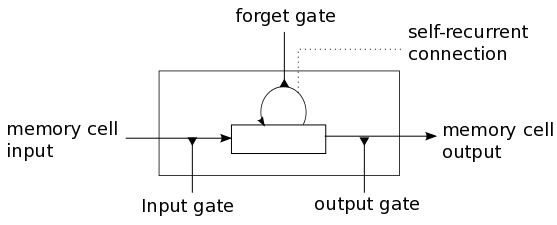
\includegraphics[width=0.75\textwidth]{img/rnn/lstm_cell.png}
	\end{tabular}
	\end{figure}
\end{frame}

%%%%%%%%%%%%%%%%%%%%%%%%%%%%%%%%%%%%%%%%%%%%%%%%%%%%%%%%%%%%%%%%%%

\begin{frame}{Long Short-Term Memory networks}
Let's see \textbf{how update equations look like for a LSTM model}. Please notice that LSTM framework, notation is usually slightly different than form vanilla RNN. 
\begin{equation}
	\begin{cases}
	\bm{i} = \sigma(\bm{x}^{(t)}\bm{U}_{i} + \bm{s}^{(t-1)}\bm{W}_{i})\\
	\bm{f} = \sigma(\bm{x}^{(t)}\bm{U}_{f} + \bm{s}^{(t-1)}\bm{W}_{f})\\
	\bm{o} = \sigma(\bm{x}^{(t)}\bm{U}_{o} + \bm{s}^{(t-1)}\bm{W}_{o})\\
	\bm{g} = \tanh(\bm{x}^{(t)}\bm{U}_g + \bm{s}^{(t-1)}\bm{W}_g)\\
	\bm{c}^{(t)} = \bm{c}^{(t-1)} \odot \bm{f} + \bm{g} \odot \bm{i}\\
	\bm{s}^{(t)} = \tanh(\bm{c}^{(t)}) \odot \bm{o}
	\end{cases}
\end{equation}
Here $\odot$ denotes element-wise multiplication. If this sounds complicated, in the following slides we'll parse each of these equations to make a sense out of it.
\end{frame}

%%%%%%%%%%%%%%%%%%%%%%%%%%%%%%%%%%%%%%%%%%%%%%%%%%%%%%%%%%%%%%%%%%

\begin{frame}{Long Short-Term Memory networks}
\begin{equation}
	\begin{cases}
	\bm{i} = \sigma(\bm{x}^{(t)}\bm{U}_{i} + \bm{s}^{(t-1)}\bm{W}_{i})\\
	\bm{f} = \sigma(\bm{x}^{(t)}\bm{U}_{f} + \bm{s}^{(t-1)}\bm{W}_{f})\\
	\bm{o} = \sigma(\bm{x}^{(t)}\bm{U}_{o} + \bm{s}^{(t-1)}\bm{W}_{o})\\
	\dots
	\end{cases}
\end{equation}\\
\vspace{0.2cm}
These are the input, forget and output \textbf{gates} respectively. Each gate has the same dimension of the hidden state. Gates are multiplied element-wise with other functions of LSTM thus acting as \textbf{continuous, differentiable switches} thanks to the sigmoid activation function.\\
\vspace{0.2cm}
\textit{Input} and \textit{output gates} controls how much of the input let through and how much of the internal state exposing to the external, respectively.	Conversely, \textit{forget gate} controls how much memory form previous time step must be overwritten.

\end{frame}

%%%%%%%%%%%%%%%%%%%%%%%%%%%%%%%%%%%%%%%%%%%%%%%%%%%%%%%%%%%%%%%%%%

\begin{frame}{Long Short-Term Memory networks}
\begin{equation}
\begin{cases}
\dots\\
	\bm{g} = \tanh(\bm{x}^{(t)}\bm{U}_g + \bm{s}^{(t-1)}\bm{W}_g)\\
	\dots\\
	\end{cases}
\end{equation}
This equation computes what could intuitively be described a \textbf{candidate state}. Indeed, the equation is pretty much the same that we saw for vanilla RNN architecture. Nonetheless, the amount of influence of $\bm{g}$ on the LSTM memory cell is controlled by input gate $\bm{i}$.
\end{frame}

%%%%%%%%%%%%%%%%%%%%%%%%%%%%%%%%%%%%%%%%%%%%%%%%%%%%%%%%%%%%%%%%%%
\begin{frame}{Long Short-Term Memory networks}
\begin{equation}
\begin{cases}
	\dots\\
	\bm{c}^{(t)} = \bm{c}^{(t-1)} \odot \bm{f} + \bm{g} \odot \bm{i}\\
	\bm{s}^{(t)} = \tanh(\bm{c}^{(t)}) \odot \bm{o}
\end{cases}
\end{equation}
First equation computes the \textbf{update for memory cell} $\bm{c}$. The \textit{forget gate} controls how much of memory from previous steps $\bm{c}^{(t)}$ must be kept. \textit{Input gate} supervises the amount of newly computed state $\bm{g}$ that has to flow into the memory.\\
\vspace{0.25cm}
Eventually, last equation compute the \textbf{output hidden state} from the current memory. \textit{Output gate} regulates the amount of information to be exposed to successive layers.
\end{frame}

%%%%%%%%%%%%%%%%%%%%%%%%%%%%%%%%%%%%%%%%%%%%%%%%%%%%%%%%%%%%%%%%%%

%%%%%%%%%%%%%%%%%%%%%%%%%%%%%%%%%%%%%%%%%%%%%%%%%%%%%%%%%%%%%%%%%%
%%%%%%%%%%%%%%%%%%%%%%%%%%%%%%%%%%%%%%%%%%%%%%%%%%%%%%%%%%%%%%%%%%
%%%%%%%%%%%%%%%%%%%%%%%%%%%%%%%%%%%%%%%%%%%%%%%%%%%%%%%%%%%%%%%%%%

\section{Credits}
\begin{frame}[t, allowframebreaks]{Credits}
These slides heavily borrow from a number of awesome sources. I'm really grateful to all the people who take the time to share their knowledge on this subject with others.\\
\vspace{0.5cm}
In particular:
\begin{itemize}
\item Stanford CS231n Convolutional Neural Networks for Visual Recognition\\
\url{http://cs231n.stanford.edu/}
\item Stanford CS20SI TensorFlow for Deep Learning Research\\
\url{http://web.stanford.edu/class/cs20si/syllabus.html}
\item Deep Learning Book (GoodFellow, Bengio, Courville)\\
\url{http://www.deeplearningbook.org/}
\item Marc'Aurelio Ranzato, "Large-Scale Visual Recognition with Deep Learning"\\
\url{www.cs.toronto.edu/~ranzato/publications/ranzato_cvpr13.pdf}
\item Convolution arithmetic animations\\
\url{https://github.com/vdumoulin/conv_arithmetic}
\item Andrej Karphathy personal blog\\
\url{http://karpathy.github.io/}
\item WildML blog on AI, DL and NLP\\
\url{http://www.wildml.com/}
\item Michael Nielsen Deep Learning online book
\url{http://neuralnetworksanddeeplearning.com/}
\end{itemize}
\end{frame}

%%%%%%%%%%%%%%%%%%%%%%%%%%%%%%%%%%%%%%%%%%%%%%%%%%%%%%%%%%%%%%%%%%
%%%%%%%%%%%%%%%%%%%%%%%%%%%%%%%%%%%%%%%%%%%%%%%%%%%%%%%%%%%%%%%%%%
%%%%%%%%%%%%%%%%%%%%%%%%%%%%%%%%%%%%%%%%%%%%%%%%%%%%%%%%%%%%%%%%%%

\begin{frame}[t, allowframebreaks]
\frametitle{References}
\bibliographystyle{abbrv}
\bibliography{bibliography}
\end{frame}
\end{document}